%
%   Chapter Experiments
%
%   Yong-Siang Shih
%   R.O.C.104.07
%
\chapter{Experiments}
\label{c:exp}

In this chapter, we discuss the evaluation for our system. Each component
is evaluated individually as well as within the pipeline system. For
statistical significance, we use Wilcoxon signed-ranks test~\citep{wilcoxon1945individual}
as suggested by \cite{demvsar2006statistical} at confidence level 0.05.

\section{Discourse Usage Disambiguation}
\label{s:discourse-usage-exp}

In this section, we describe our investigation
on discourse usage disambiguation. We evaluate our models using
10-fold cross-validation. The 2,342 paragraphs are divided  into 10 splits
while keeping the distribution for the number of explicit relations
in each paragraph roughly equal. Most of the related works only
deal with connective components, so we will also use the 2,131 annotated
components to evaluate our models.
The precision, recall, and F1 score for the positive instances are computed
for each fold, and the averaged results are reported.

In Section~\ref{s:linking-exp}, we will also investigate whether solving linking
ambiguities could improve the discourse usage disambiguation. The results
are summarized, and comparison with with other works is presented.


\subsection{Disambiguation on Component Level}

We firstly evaluate disambiguation on component level as specified in
Section~\ref{s:discourse-disambig-component}.  
Different types of word embeddings for
the VECTOR features are experimented. We use Logistic Regression
as our classifier with VECTOR as the only features. The results are
shown in Table~\ref{t:recognition-vectors} below. 

\begin{table}[ht]
\centering
\begin{tabular}{|l|c|c|c|}
\hline

    Features        &     Precision &     Recall &     F1-Score \\ \hline
    GLOVE           &     77.95     &     75.77  &     76.79    \\ \hline
    SKIPGRAM        & \bf 78.33     &     76.28  & \bf 77.25    \\ \hline
    CBOW            &     75.08     &     73.97  &     74.48    \\ \hline
    GLOVE+SKIPGRAM  &     77.82     & \bf 76.57  &     77.15    \\ \hline
    GLOVE+CBOW      &     74.63     &     73.79  &     74.14    \\ \hline
    SKIPGRAM+CBOW   &     74.56     &     73.55  &     74.01    \\ \hline
    All             &     74.91     &     73.46  &     74.12    \\ \hline

\end{tabular}
\caption{\label{t:recognition-vectors} Performance of discourse usage
disambiguation on component level using different word embeddings for
the VECTOR features. }
\end{table}


GLOVE is trained with the Glove toolkit~\citep{pennington2014glove}
while SKIPGRAM and CBOW are trained using word2vec~\citep{mikolov2013efficient} with
continuous skip-gram and continuous bag-of-words models,
respectively. SKIPGRAM yields the best results.
We have tried concatenating different embeddings
but the performance does not improve. Therefore, we will only use SKIPGRAM
for the remaining experiments.

We also use the same 10-fold to evaluate different features we proposed.
The results are shown in Table~\ref{t:recognition-features}. SIKIPGRAM
is the most powerful feature set. Combining all features yields the best results.

\begin{table}[!htbp]
\centering
\begin{tabular}{|l|c|c|c|}
\hline

Features        &     Precision &     Recall &     F1-Score                 \\ \hline
P \& N          &     74.52     &     45.02  &     55.96\textsuperscript{*} \\ \hline
POS             &     75.47     &     65.76  &     70.24\textsuperscript{*} \\ \hline
NUM             &     68.39     &     22.20  &     33.30\textsuperscript{*} \\ \hline
SKIPGRAM        &     78.33     &     76.28  &     77.25\textsuperscript{*} \\ \hline
All-P \& N      &     79.09     &     76.97  &     77.99\textsuperscript{*} \\ \hline
All-POS         &     78.90     &     76.64  &     77.73\textsuperscript{*} \\ \hline
All-NUM         &     79.42     & \bf 77.44  &     78.40\textsuperscript{ } \\ \hline
All-SKIPGRAM    &     77.89     &     68.70  &     72.96\textsuperscript{*} \\ \hline
All             & \bf 79.92     & \bf 77.44  & \bf 78.64\textsuperscript{!} \\ \hline


\end{tabular}
\caption{\label{t:recognition-features} Performance of discourse usage
disambiguation on component level using different features. }
\end{table}


We use Scikit-Learn library~\citep{scikit-learn} to experiment with
several learning models with default parameters using all features.
Table~\ref{t:recognition-models} shows the results. The F1 score for Logistic
Regression is the highest.


\begin{table}[ht]
\centering
\begin{tabular}{|l|c|c|c|}
\hline

    Model                  &     Precision &     Recall &     F1-Score \\ \hline
    Gaussian Naive Bayes   &     42.35     & \bf 92.17  &     58.02    \\ \hline
    SVM with RBF kernel    &     80.00     &     69.84  &     74.55    \\ \hline
    SVM with linear kernel &     75.82     &     74.66  &     75.21    \\ \hline
    Decision Tree          &     74.56     &     73.47  &     73.98    \\ \hline
    Random Forest          & \bf 82.82     &     71.39  &     76.64    \\ \hline
    Logistic Regression    &     79.92     &     77.44  & \bf 78.64    \\ \hline

\end{tabular}
\caption{\label{t:recognition-models} Performance of discourse usage
disambiguation on component level using different learning models. }
\end{table}


\subsection{Disambiguation on Connective Level}

We continue to  evaluate disambiguation on connective level as specified in
Section~\ref{s:discourse-disambig-connective}. For evaluation on component instances,
we take the union of all connective components the resulting connective candidates
have as the final result for evaluation.

Table~\ref{t:recognition-connective-features} shows the results with different features.
As there remain many overlapped candidates, the precision for connective instances
are relatively low compared to the precision for component instances. The best performance
for component instances is slightly higher than that of disambiguation on component level in
Table~\ref{t:recognition-features},
but the difference is insignificant.

%t:recognition-connective-features
\begin{table}[ht]
\centering
\begin{tabular}{|l|c|c|c|c|c|c|}
\hline
                    & \multicolumn{3}{c|}{Connective Instances}  & \multicolumn{3}{c|}{Component Instances}  \\ \hline
    Features        &     Precision &     Recall &     F1-Score  &     Precision &     Recall &     F1-Score \\ \hline
    P \& N          &     42.39     &     84.09  &     56.34     &     53.33     &     82.77  &     64.83    \\ \hline
    POS             &     54.26     &     78.05  &     63.99     &     65.65     &     77.83  &     71.19    \\ \hline
    NUM             &     43.00     & \bf 84.62  &     56.99     &     49.47     & \bf 84.05  &     62.25    \\ \hline
    SKIPGRAM        &     60.13     &     80.68  &     68.87     &     73.23     &     79.46  &     76.19    \\ \hline
    All-P \& N      &     64.51     &     82.05  &     72.17     &     74.76     &     80.74  &     77.60    \\ \hline
    All-POS         &     64.98     &     82.16  &     72.54     &     74.93     &     81.01  &     77.83    \\ \hline
    All-NUM         &     62.09     &     81.50  &     70.46     &     75.48     &     80.63  &     77.95    \\ \hline
    All-SKIPGRAM    &     57.15     &     81.96  &     67.31     &     66.06     &     80.85  &     72.68    \\ \hline
    All             & \bf 66.13     &     82.44  & \bf 73.37     & \bf 76.23     &     81.35  & \bf 78.68    \\ \hline

\end{tabular}
\caption{\label{t:recognition-connective-features} Performance of discourse usage
disambiguation on connective level using different features. }
\end{table}


We also experiment with different learning models and the results
in Table~\ref{t:recognition-connective-models} are similar to that of disambiguation on
component level.

%t:recognition-connective-models
\begin{table}[ht]
\centering
\begin{tabular}{|l|c|c|c|c|c|c|}
\hline
                            & \multicolumn{3}{c|}{Connective Instances} & \multicolumn{3}{c|}{Component Instances}  \\ \hline
\bf Model                   & \bf Precision & \bf Recall & \bf F1-Score  & \bf Precision & \bf Recall & \bf F1-Score \\ \hline
    Gaussian Naive Bayes    &     34.17     & \bf 94.68  &     50.20     &     41.84     & \bf 92.74  &     57.65    \\ \hline
    SVM with RBF kernel     &     58.38     &     87.90  &     70.15     &     69.40     &     85.26  &     76.46    \\ \hline
    SVM with linear kernel  &     64.80     &     78.80  &     71.10     &     74.40     &     77.75  &     76.02    \\ \hline
    Decision Tree           &     70.03     &     66.99  &     68.43     &     76.23     &     66.24  &     70.84    \\ \hline
    Random Forest           & \bf 73.06     &     68.49  &     70.69     & \bf 82.48     &     67.11  &     73.97    \\ \hline
    Logistic Regression     &     66.13     &     82.44  & \bf 73.37     &     76.23     &     81.35  & \bf 78.68    \\ \hline

\end{tabular}
\caption{\label{t:recognition-connective-models} Performance of discourse usage
disambiguation on connective level using different learning models. }
\end{table}



\section{Discourse Linking Disambiguation}
\label{s:linking-exp}

In this section, we discuss our investigation on linking ambiguities between connective
components. Evaluation is done by calculating the precision, recall, and F1 for the
1,813 connective instances.
The same 10-fold for paragraphs is used for the experiments.

\subsection{Discourse Linking Disambiguation for Known Connective Components}

We start by evaluating linking resolution individually by assuming all correct
connective components are already known. The results are reported in
Table~\ref{t:linking-perfect-methods}.
We evaluate different ranking criteria such as scores predicted by
Logistic Regression, the lengths of the connective candidates, and the combination
of the two. Ties are broken by the positions of the connective candidates.
Baseline models that only rank the candidates by their positions are also reported.

We found that the ambiguity among the components is low. The simple
baseline model already achieves an F1 of 87.97\%. The greedy
Algorithm~\ref{a:linking-resolve} could improve the baseline
model significantly, but once ranking is employed, it doesn't contribute much.
The difference for F1 between \textit{score+} and \textit{len+} is statistically
significant, but the difference between \textit{score+} and \textit{len-score+}
is insignificant.

%t:linking-perfect-methods
\begin{table}[ht]
\centering
\begin{tabular}{|l|c|c|c|}
\hline
                        & \multicolumn{3}{c|}{Connective Instances}                 \\ \hline
Method                  &     Precision &     Recall &     F1-Score                 \\ \hline
baseline+               &     87.65     &     93.28  &     90.38\textsuperscript{*} \\ \hline
len+                    &     97.60     &     96.04  &     96.81\textsuperscript{*} \\ \hline
score+                  &     97.37     & \bf 97.57  & \bf 97.47\textsuperscript{!} \\ \hline
len-score+              & \bf 98.15     &     96.59  &     97.36\textsuperscript{ } \\


\hhline{|=|=|=|=|}

baseline                &     85.28     &     90.84  &     87.97\textsuperscript{*} \\ \hline
len                     &     97.60     &     96.04  &     96.81\textsuperscript{*} \\ \hline
score                   &     97.26     &     97.46  &     97.36\textsuperscript{ } \\ \hline
len-score               & \bf 98.15     &     96.59  &     97.36\textsuperscript{ } \\ \hline

\end{tabular}
\begin{flushleft}
\small
\textbf{+}: greedily accept connectives with linking ambiguity $=$ 1
\end{flushleft}
\caption{\label{t:linking-perfect-methods} Performance of linking
disambiguation with known connective components. }
\end{table}




\cite{hu2011research} evaluated their algorithm on 79 sentences that have
linking ambiguities, and they correctly resolved all linking ambiguities for 78
sentences. In our corpus, there are 52 paragraphs that have linking ambiguity
and are composed of only 1 sentence. We evaluate our non-learning \text{len+} model
directly on these 52 sentences and are able to correctly resolve all linking
ambiguities in 51 sentences. Our relatively simple greedy algorithm is
able to achieve similar results when the components are known.

\subsection{Discourse Linking Disambiguation within Pipeline System}

For practical applications, it's difficult to know which component is correct in
advance. Therefore, we also evaluate linking disambiguation within the pipeline
system. The results are shown in Table~\ref{t:linking-methods}. Unlike the case
when all components are known, accepting candidates with linking ambiguity $=$ 1 actually
decreases the performance.

In addition, alternative approaches using discourse usage
disambiguation on component level and connective
level as described in Section~\ref{s:discourse-disambig-component} and
Section~\ref{s:discourse-disambig-component} are compared.
Although it is not statistically significant, for both connective
instances and components instances, the best results for disambiguation on connective
level are higher to that for disambiguation on component level.
In addition, it is also relatively computation-efficient as the same Logistic
Regression predictions are used for both discourse usage disambiguation and ranking.
Therefore, we choose the \textit{\#len-score} model for the next stage of our
pipeline system.

%t:linking-methods
\begin{table}[ht]
\centering
\begin{tabular}{|l|c|c|c|c|c|c|}
\hline
            & \multicolumn{3}{c|}{Connective Instances}                 & \multicolumn{3}{c|}{Component Instances}                  \\ \hline
Method      &     Precision &     Recall &     F1-Score                 &     Precision &     Recall &     F1-Score                 \\ \hline
@baseline+  &     74.23     &     66.05  &     69.88\textsuperscript{*} &     82.30     &     72.98  &     77.33\textsuperscript{*} \\ \hline
@len+       &     78.15     &     68.82  &     73.18\textsuperscript{*} & \bf 83.26     &     70.40  &     76.27\textsuperscript{*} \\ \hline
@score+     &     75.47     &     70.79  &     73.04\textsuperscript{*} &     82.18     &     72.28  &     76.89\textsuperscript{*} \\ \hline
@len-score+ & \bf 78.92     &     69.49  &     73.89\textsuperscript{*} &     83.08     &     70.77  &     76.41\textsuperscript{*} \\

\hhline{|=|=|=|=|=|=|=|}

@baseline   &     68.25     &     69.70  &     68.96\textsuperscript{*} &     81.03     &     73.64  &     77.13\textsuperscript{*} \\ \hline
@len        &     74.53     &     71.09  &     72.75\textsuperscript{*} &     81.29     &     75.20  &     78.10\textsuperscript{*} \\ \hline
@score      &     73.79     &     72.40  &     73.07\textsuperscript{*} &     81.75     &     75.24  &     78.33\textsuperscript{ } \\ \hline
@len-score  &     75.66     &     72.08  &     73.81\textsuperscript{ } &     81.84     &     75.66  &     78.60\textsuperscript{ } \\

\hhline{|=|=|=|=|=|=|=|}

\#baseline+ &     69.25     &     73.06  &     71.09\textsuperscript{*} &     77.42     &     75.04  &     76.19\textsuperscript{*} \\ \hline
\#len+      &     74.21     &     74.11  &     74.15\textsuperscript{ } &     78.26     &     76.90  &     77.55\textsuperscript{*} \\ \hline
\#score+    &     71.75     &     75.20  &     73.41\textsuperscript{*} &     77.60     &     78.89  &     78.21\textsuperscript{*} \\ \hline
\#len-score+&     74.57     &     74.72  &     74.63\textsuperscript{ } &     78.38     &     78.11  &     78.23\textsuperscript{ } \\

\hhline{|=|=|=|=|=|=|=|}

\#baseline  &     68.09     &     73.45  &     70.65\textsuperscript{*} &     76.84     &     77.19  &     76.99\textsuperscript{*} \\ \hline
\#len       &     72.84     &     76.25  &     74.49\textsuperscript{ } &     76.82     &     79.98  &     78.35\textsuperscript{*} \\ \hline
\#score     &     71.71     &     75.86  &     73.71\textsuperscript{*} &     77.59     &     79.35  &     78.44\textsuperscript{ } \\ \hline
\#len-score &     73.30     & \bf 76.75  & \bf 74.97\textsuperscript{!} &     77.27     & \bf 80.45  & \bf 78.81\textsuperscript{!} \\ \hline

\end{tabular}
\begin{flushleft}
\small
\textbf{@}: disambiguation on component level \\
\textbf{\#}: disambiguation on connective level \\
\textbf{+}: greedily accept connectives with linking ambiguity $=$ 1
\end{flushleft}
\caption{\label{t:linking-methods} Performance of linking
disambiguation for different methods. }
\end{table}



Since discourse disambiguation is not directly optimized together with linking
disambiguation, we also try to adjust the threshold for the Logistic Regression
to eliminate the candidates when using disambiguation on connective level to see if
it affects the performance, and we found that our model
obtains similar F1 scores across different thresholds as
shown in Figure~\ref{i:classify-threshold}.

%i:classify-threshold
\begin{figure}[!htbp]
\centering
    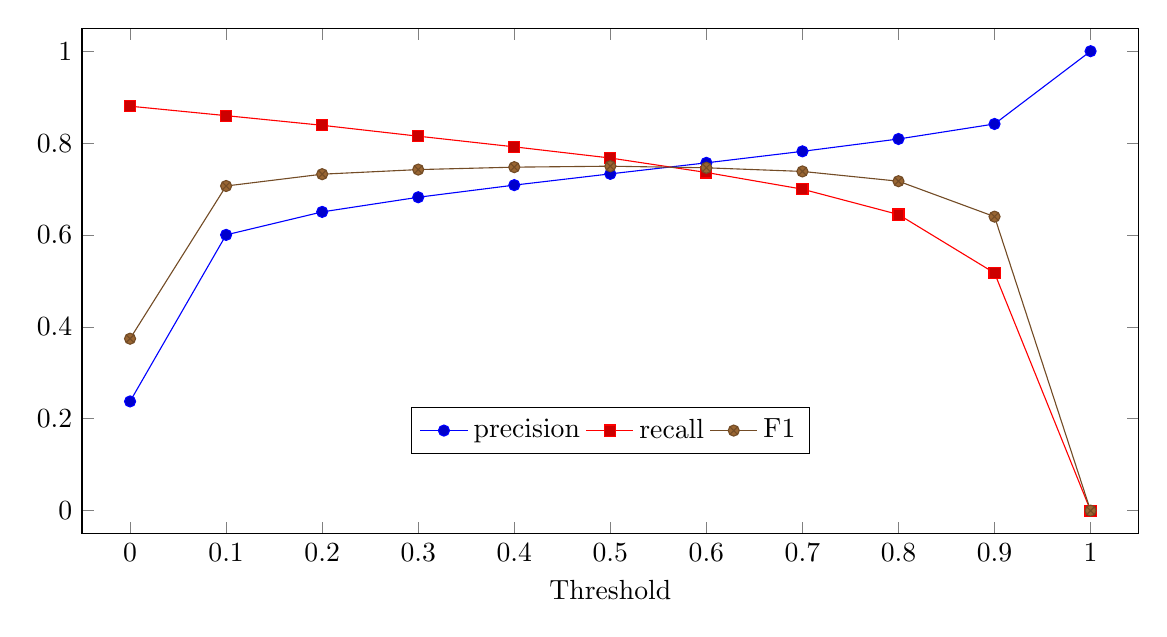
\begin{tikzpicture}
        \begin{axis}[
                height=8cm,
                width=15cm,
                xlabel=Threshold,
                legend style={at={(0.5,0.25)},
                anchor=north,legend columns=-1},
                enlarge x limits=0.05,
                enlarge y limits=0.05,
                xticklabel style={/pgf/number format/assume math mode},
                yticklabel style={/pgf/number format/assume math mode},
            ]
            \addplot+[sharp plot] coordinates
            {
                (0.0,0.2377)
                (0.1,0.6002)
                (0.2,0.6502) 
                (0.3,0.6821) 
                (0.4,0.7085) 
                (0.5,0.7330)
                (0.6,0.7570) 
                (0.7,0.7820) 
                (0.8,0.8089) 
                (0.9,0.8416) 
                (1.0,1.0000)};

            \addplot+[sharp plot] coordinates
            {
                (0.0,0.8803)
                (0.1,0.8597) 
                (0.2,0.8387) 
                (0.3,0.8150) 
                (0.4,0.7918) 
                (0.5,0.7675)
                (0.6,0.7360) 
                (0.7,0.6997) 
                (0.8,0.6445) 
                (0.9,0.5172) 
                (1.0,0.0000)};

            \addplot+[sharp plot] coordinates
            {
                (0.0,0.3742)
                (0.1,0.7066) 
                (0.2,0.7323) 
                (0.3,0.7423) 
                (0.4,0.7476) 
                (0.5,0.7497)
                (0.6,0.7462) 
                (0.7,0.7383) 
                (0.8,0.7170) 
                (0.9,0.6399) 
                (1.0,0.0000)};

            \legend{precision,recall,F1}
        \end{axis}
    \end{tikzpicture}
\caption{\label{i:classify-threshold} Performance for the pipeline system
with different thresholds. }
\end{figure}


Finally, We summarize our results for discourse disambiguation for
connective component instances in Table~\ref{t:recognition-methods}. We also
compare with various related work. The first two models are discourse disambiguation
on component level and on connective level without linking resolution. The following
models eliminates additional candidates by resolving linking ambiguity.
Some spurious candidates are removed in this process. However, it also removes some
correct components, so the resulting F1 score does not improve much.

%t:recognition-methods
\begin{table}[ht]
\centering
\begin{tabular}{|l|c|c|c|c|}
\hline

    Method                    &     Precision &     Recall &     F1-Score &     Accuracy \\ \hline
    @ w/o linking resolution  &     79.92     &     77.44  &     78.64    &     92.79    \\ \hline
    \# w/o linking resolution &     76.23     &     81.35  &     78.68    &     92.46    \\ \hline
    @len-score                & \bf 81.84     &     75.66  &     78.60    & \bf 92.96    \\ \hline
    \#len-score               &     77.27     &     80.45  &     78.81    &     92.61    \\

\hhline{|=|=|=|=|=|}

    Li et al. maximum entropy &     78.8      &     61.8   &     69.2     &     87.2     \\ \hline
    Li et al. decision tree   &     56.8      &     49.6   &     52.3     &     88.4     \\

\hhline{|=|=|=|=|=|}

    Zhou et al.               &               &            &     79.33    &     70.43    \\ \hline
    J. Jessy Li et al.        &     78.57     & \bf 81.48  & \bf 80.00    &     82.04    \\ \hline

\end{tabular}
\begin{flushleft}
\small
\textbf{@}: disambiguation on component level \\
\textbf{\#}: disambiguation on connective level \\
\end{flushleft}
\caption{\label{t:recognition-methods} Comparison for performance of discourse usage
disambiguation for connective component instances. }
\end{table}


We also compare our results with the models from \cite{li2015automatic} as they use the
same dataset as us. The best results for Maximum Entropy and Decision Tree classifiers with
automatic parsing tree features are selected. We use the 12,526 connective components candidates
extracted by string matching with connective lexicon as our basis to compute the accuracy in order
to compare with their work. Our models perform significantly better by a large margin.

We also list the results from \cite{zhou2012cross} and \cite{li2014cross} on different
datasets. Though it's not directly comparable with our work, the performance for F1 is similar,
and we have better accuracy.


\section{Discourse Relation Disambiguation}

In this section, we discuss the evaluation on discourse relation disambiguation.

\subsection{Discourse Relation Disambiguation for Known Connectives}

We will first evaluate our models using 10-fold cross-validation with the 1,813
explicit connectives. We divide them into 10 splits
while keeping the distribution for the relation types roughly equal for
each fold. We use Logistic Regression to classify the relation types.
Two sets of experiments for the disambiguation on the four top-level
categories and the 17 second-level categories are examined. The macro-averaged
precision, recall, and F1 for different relation types and the accuracy for
all instances are computed. Since many of the 17 categories occur less than
10 times in the corpus, we ignore a relation type when computing macro-averaged
scores if it does not appear in the testing fold. The averaged results over
the 10 folds are shown in Table~\ref{t:sense-features}.

We examined whether the same features
for connective candidates specified in Section~\ref{s:connective-features} are
also useful for relation type disambiguation. In addition, we use the string
of the connective itself as a feature. While the NUM features have some
discriminative power for discourse usage disambiguation on connective level,
it does not help for relation disambiguation. SKIPGRAM is still the most powerful
feature set.

%t:sense-features
\begin{table}[ht]
\centering
\begin{tabular}{|l|c|c|c|c|c|c|c|c|}
\hline
                  & \multicolumn{4}{c|}{4 Relation Types}      & \multicolumn{4}{c|}{17 Relation Types}                                    \\ \hline
\bf Features      & \bf P         & \bf R      & \bf F         & \bf A         & \bf P         & \bf R      & \bf F        & \bf A         \\ \hline
    P \& N        &     94.94     &     91.85  &     93.08     &     79.98     &     71.32     &     61.72  &     64.42    &     86.53     \\ \hline
    POS           &     85.66     &     70.47  &     75.10     &     82.79     &     34.51     &     31.12  &     31.76    &     68.58     \\ \hline
    NUM           &     13.42     &     24.97  &     17.46     &     53.67     &      8.24     &      7.27  &      4.99    &     41.27     \\ \hline
    SKIPGRAM      &     95.23     &     94.43  &     94.73     &     95.36     &     77.36     &     72.36  & \bf 73.40    &     89.02     \\ \hline
    CONNECITVE    &     94.94     &     91.85  &     93.08     &     94.16     &     71.32     &     61.72  &     64.42    &     86.53     \\ \hline
    All-P \& N    &     95.33     &     94.39  &     94.77     &     95.59     &     74.07     &     67.60  &     69.20    &     88.73     \\ \hline
    All-POS       &     95.51     &     94.12  &     94.70     &     95.36     &     71.04     &     66.31  &     67.42    &     88.13     \\ \hline
    All-NUM       & \bf 95.84     &     94.52  &     95.07     &     95.80     & \bf 75.69     & \bf 72.38  &     73.16    & \bf 89.23     \\ \hline
    All-SKIPGRAM  &     94.69     &     92.76  &     93.58     &     94.88     &     68.63     &     62.58  &     64.00    &     86.54     \\ \hline
    All-CONNECITVE&     95.44     &     94.47  &     94.86     &     95.64     &     71.77     &     66.15  &     67.50    &     88.30     \\ \hline
    All           &     95.77     & \bf 94.78  & \bf 95.18     & \bf 95.97     &     71.49     &     66.96  &     68.01    &     88.52     \\ \hline

\end{tabular}
\caption{\label{t:sense-features} Performance of relation type
disambiguation for connectives by different features. }
\end{table}



In Table~\ref{t:sense-types}, we show the performance for different relation types
using All-NUM as features. For the second-level relation types, we only list
those type that have more than 10 instances. We could notice that the
number of instances affects the performance of the learning model. The
lesser the instances, the worse the performance.

%t:sense-types
\begin{table}[ht]
\centering
\begin{tabular}{|l|c|c|c|c|}
\hline

\multicolumn{5}{|c|}{4 Relation Types}                                              \\ \hline
    Features            &     Precision &     Recall &     F1-Score &     Instances \\ \hline
    causality           &     96.34     &     95.04  &     95.61    &     465       \\ \hline
    coordination        &     95.75     &     97.23  &     96.45    &     974       \\ \hline
    transition          &     93.72     &     91.31  &     92.34    &     173       \\ \hline
    explanation         &     97.54     &     94.50  &     95.88    &     201       \\ \hline
    macro-AVG           &     95.84     &     94.52  &     95.07    &     1813      \\ \hline

\multicolumn{5}{|c|}{14 Relation Types}                                             \\ \hline
    Features            &     Precision &     Recall &     F1-Score &     Instances \\ \hline
    cause-result        &     89.71     &     94.57  &     91.98    &     203       \\ \hline
    hypothetical        &     92.17     &     86.00  &     88.65    &     55        \\ \hline
    purpose             &     94.18     &     88.27  &     90.91    &     163       \\ \hline
    condition           &     75.50     &     66.67  &     68.60    &     37        \\ \hline
    coordination        &     88.10     &     96.22  &     91.95    &     741       \\ \hline
    continue            &     84.22     &     74.18  &     78.35    &     133       \\ \hline
    progressive         &     84.50     &     55.67  &     65.25    &     52        \\ \hline
    selectional         &     50.00     &     50.00  &     50.00    &     10        \\ \hline
    inverse             &     76.67     &     28.33  &     39.71    &     38        \\ \hline
    transition          &     92.00     &     91.17  &     91.46    &     157       \\ \hline
    concessive          &     80.00     &     75.00  &     76.67    &     16        \\ \hline
    explanation         &     55.00     &     60.00  &     56.67    &     11        \\ \hline
    summary-elaboration &     99.38     &     98.12  &     98.73    &     158       \\ \hline
    example             &     87.50     &     90.00  &     87.90    &     29        \\ \hline
    macro-AVG           &     82.07     &     75.30  &     76.92    &     1803      \\ \hline

\end{tabular}
\caption{\label{t:sense-types} Performance of relation type
disambiguation. }
\end{table}


%t:sense-types-pipeline
\begin{table}[ht]
\centering
\begin{tabular}{|l|c|c|c|c|}
\hline

\multicolumn{5}{|c|}{4 Relation Types}                                              \\ \hline
\bf Features            & \bf Precision & \bf Recall & \bf F1-Score & \bf Instances \\ \hline
    causality           &     69.98     &     75.37  &     72.24    &     465       \\ \hline
    coordination        &     67.70     &     70.63  &     69.09    &     974       \\ \hline
    transition          &     80.75     &     76.31  &     78.25    &     173       \\ \hline
    explanation         &     80.84     &     89.27  &     84.49    &     201       \\ \hline
    macro-AVG           &     74.82     &     77.90  &     76.02    &     1813      \\ \hline
    micro-AVG           &     71.13     &     74.48  &     72.75    &     1813      \\ \hline

\end{tabular}
\caption{\label{t:sense-types-pipeline} Performance of relation type
disambiguation within the pipeline system. }
\end{table}


We also investigate end-to-end.

\section{Explicit Discourse Relation Argument Extraction}
